\documentclass[preprint]{aastex}
\usepackage{graphicx}
\usepackage{natbib}
\usepackage{wrapfig}
\usepackage{amsmath}
\usepackage{simplemargins}
%\setallmargins{0.8in}
\setleftmargin{0.75in}
\setrightmargin{0.75in}
\settopmargin{0.72in}
\setbottommargin{0.72in}
\bibliographystyle{apj}
\pagestyle{plain}

\renewcommand{\abstractname}{Summary}
\newcommand\etal{{\it et al.}}
\newcommand\eg{{\it e.g.,~}}
\newcommand\ie{{\it i.e.,~}}

\begin{document}

\title{\LARGE \bf Numerical Simulations of Turbulence in an Accretion Disk with a Vertical Temperature Gradient}
\author{\large Daniel A. Gole, Jacob B. Simon}
\affil{JILA/University of Colorado, Boulder}
\maketitle
\vspace{-8mm}
\section{Summary}
We request $\mathbf{4.29\times10^6}$ {\bf SUs} on the {\sc Summit} supercomputer to conduct numerical simulations of astrophysical accretion disks around young stars.
Utilizing the well-tested, publicly available, magnetohydrodynamics code {\sc Athena}, we will evolve local, co-rotating regions of these disks to explore the effect of a vertical temperature gradient on the turbulence and turbulent transport in the disk.  Funding for the proposed research will be provided by... 

\vspace{-8mm}
\section{Introduction and Scientific Motivation}
\vspace{-2mm}
Disks around young stars play a crucial role in star and planet formation processes.  These {\it protoplanetary disks} actively accrete their gas onto the central star, contributing to the young star's growth, and contain the rocky building blocks for planets to form.  
Both the accretion of gas onto the star and the processes that produce planets are intimately tied to {disk turbulence} driven by the magnetorotational instability \cite[MRI;][]{balbus91,balbus98}.  

In fully ionized disks, such as those around black holes, the MRI is very efficient at producing turbulence and driving accretion.  However, protoplanetary disks are significantly colder than their black hole counterparts and consequently have a lower ionization fraction throughout large regions of the disk.  Since strong coupling of the gas to magnetic fields is crucial for the MRI to operate, there can be extensive regions of no MRI activity in such disks.  In fact, for radial distances larger than $\sim$0.1 AU, the temperature of the gas is simply too low for thermal ionization \citep{umebayashi83}.  Instead, the disk surface layers (far from the disk mid-plane) are ionized by cosmic rays \citep{gammie96}, stellar X-rays \citep{igea99}, and stellar FUV photons \citep{perez-becker11b}.  In the outer regions of the disk, the dominant non-ideal MHD effect from the large fraction of neutrals is ambipolar diffusion \citep{armitage11,turner14}.  The current paradigm for accretion in this situation is a layered disk model, with most of the accretion occuring in the ionized and turbulent outer layers and little to no accretion at the mid-plane of the disk.

In conflict with this paradigm are recent observations of the protoplanetary disk HD 163296 \citep{Flaherty15}.  This study uses spectral line widths to measure the non-thermal motions (turbulence) in the outer layer of the disk and finds that the motions are about an magnitude slower than expected from simulations.  

One factor that has not been well studied in 3D simulations is the vertical temperature profile of the disk.  This will likely have an effect on the turbulence as a function of height, and may explin the "weak turbulence problem" observed by \cite{Flaherty15}.  In the outer regions of the disk (large radii), the temperature profile is determined primarily by radiation heating the upper layer of the disk.  This energy then progagates twoards the mid-plane, where it is cooler.  We will use the temperature profile model proposed by \citep{temperatureProfile} in this study and examine the effect that it has on the turbulence as a function of height.              

\vspace{-8mm}
\section{Proposed Simulations}
\vspace{-2mm}

We will perform local "shearing-box" simulations of a small, co-rotating patch of a protoplanetary disk.  These simulations will include a simple ionization profile model that gives rise to ambipolar diffusion.  The novel piece of physics included in these simulations will be adiabiticity and a temperature gradient in the $z$ direction.  This control parameters of the study are all related to the temperature profile.  The gas in our shearing box will heat and cool twoards an equilibrium temperature profile \citep{temperatureProfile} with a characteristic cooling time.  We intend to carry out 9 simulations.  The main parameter to be explored will be the ratio of the temperature in the atmosphere of the disk (high $|z|$) to the temperature at the mid-plane of the disk ($z=0$): $T_{atm}/T_{mid}$.  This will change the vertical temperature gradient within the disk, and most of our analysis will be focused on how this gradient changes the turbulence relative to a vertically isothermal disk.  As a control study, we will also consider the case where $T_{atm}/T_{mid}=1.0$ (no gradient, but adiabatic perturbations).  As another control, we will also consider the truly isothermal case.  One of the less constrained parameters in this study is the cooling time, so we will also consider several different cooling times.  We do not expect this to have a large effect on the results of the study, but it is worthwhile to show that to be true.  All parameters related to the ionization state of the disk as a function of height will be held constant over all simulations.  Table 1 shows the proposed parameters for all of the simulations.  

The resolution required to resolve the relevant phenomena is primarily limited by the characteristic wavelength of the magnetorotational instability.  For the parameters we will be using, the wavelength is about $0.2H$, where $H$ is the pressure scalce height of the disk.  We plan to use a resolution of 60 zones per $H$, which gives us about 11 zones per MRI wavelength and will be sufficient to resolve the instability and drive turbulence.  

\vspace{5mm}
\begin{deluxetable}{c c c c c c c}
\label{table}
%\tabletypesize{\small}
\tablecaption{Proposed Simulations}
\tablewidth{\textwidth}
\startdata
\hline \hline
Equation of State & Cooling Time & $T_{atm}/T_{mid}$ & zones & orbits & SU's \\
\hline
Isothermal & n/a & n/a  & $120 \times 240 \times 480$ & 100 & $2.01 \times 10^5$ \\
Adiabatic  & 0.1 & 0.01 & $120 \times 240 \times 480$ & 100 & $2.01 \times 10^5$ \\
Adiabatic  & 0.1 & 0.1  & $120 \times 240 \times 480$ & 100 & $2.01 \times 10^5$ \\
Adiabatic  & 0.1 & 0.5  & $120 \times 240 \times 480$ & 100 & $2.01 \times 10^5$ \\
Adiabatic  & 0.1 & 1.0  & $120 \times 240 \times 480$ & 100 & $2.01 \times 10^5$ \\
Adiabatic  & 0.1 & 3.0  & $120 \times 240 \times 480$ & 100 & $2.01 \times 10^5$ \\
Adiabatic  & 0.1 & 0.5  & $120 \times 240 \times 480$ & 100 & $2.01 \times 10^5$ \\
Adiabatic  & 0.1 & 0.5  & $120 \times 240 \times 480$ & 100 & $2.01 \times 10^5$ \\
Adiabatic  & 0.1 & 0.5  & $120 \times 240 \times 480$ & 100 & $2.01 \times 10^5$ \\
\hline
%\vspace{-1mm}
 & & & & {\bf Total} & {$\bf 1.81\times10^6$ {\bf SUs}} \\
\enddata
\end{deluxetable}


\vspace{-8mm}
\section{Computational Methods}
\label{sec:code}
\vspace{-2mm}

Our simulations will use the publicly available and extensively tested multidimensional MHD code {\sc Athena}.  The fundamental structure of {\sc Athena} is described in \citet{gardiner05a} and \citet{gardiner08} with detailed descriptions of the algorithms appearing in \citet{stone08} and \cite{stone10}.
For this project, we will be using {\sc Athena}, as presented in \citet{stone10}, to solve the equations of compressible MHD in the shearing box limit with and adiabatic equation of state and Ambipolar diffusion, which is responsible for the dead zone. 
This is accomplished with a dimensionally unsplit, second-order accurate integrator combined with a constrained transport method for evolving the magnetic induction equation and preserving a divergence-free magnetic field. 
Additionally, as elaborated upon in \citet{stone10}, certain modifications have been made to the code in the shearing box approximation in order to conserve vertical magnetic flux to machine precision, as well as to accurately capture the physics of epicyclic motion.  An orbital advection scheme has also been implemented to remove numerical diffusion created by the Keplerian shear flow and to increase the Courant limited time step.

{\sc Athena} is parallelized via domain decomposition through MPI.  The code has been optimized so that the number of MPI communication calls is on the order of once per time step; this leads to excellent scaling on large numbers of cores.  In the following section we describe how we have tested and optimized for use on {\sc Summit}



\vspace{-8mm}
\section{Optimization for Summit and Justification of Compute Resources}
\vspace{-2mm}

CHANGE ALL OF THIS ONCE IT GETS SORTED OUT.  Strong and weak scaling tests were performed on {\sc Summit}, the results are show in Figure 1.  The strong scaling test indicates that we can go down to about $20^3$ zones per MPI domain without sacrificing speed. The weak scaling tests were somewhat dissapointing on {\sc Summit} when compared to similar tests on other machines.  Relative to an 8 core job, a 512 core job is 41\% as effecient, and a 1000 core job is 0.5\% as effecient (normalized to the number of cores).  For this reason, we will limit jobs to 512 cores (22 nodes) and will not go below $20^3$ zones per core.  

Several compiler options were tried, with the best results being plotted.  
  
\begin{figure}[h]
\label{figScaling}
\vspace{-0.3cm}
\begin{center}
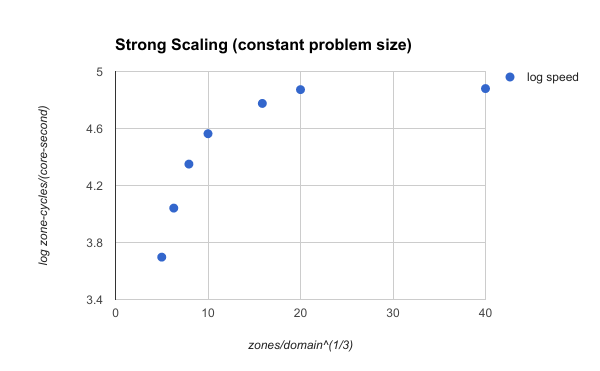
\includegraphics[width=75mm]{./strongScaling.png}
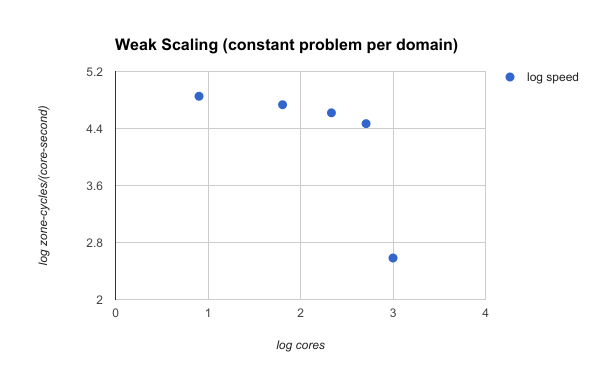
\includegraphics[width=75mm]{./weakScaling.png}
\vspace{-0.3cm}
\caption{Strong and weak scaling tests.}
\end{center}
\vspace{-0.6cm}
\label{fig:weakScaling}
\end{figure}

For the 1296-core simulations we propose, the performance has been about $6 \times 10^4$ zone-cycles/(core-second).  Extrapolating from tests at lower resolution, we estimate that about $3 \times 10^4$ cycles are required to evolve for one orbit. These numbers are used to calculate the total required SU for each run in Table 1.  


\vspace{-8mm}
\section{I/O and Justification of Storage Resources}
\vspace{-2mm}

We will output 3 different file types:
\begin{itemize}
\item 3D table files contain the full 3D data dump at one point in time and will be used to carry out most of the analysis.  These files are output core-by-core, each core writing to it's own directory.  These will be 1.4MB per core per output, for a total of $1.4 \times 1728$MB$=2.42$GB per full data dump.  We will output this once per orbit.
\item  Restart files are a full 3D data dump that can be used to resume the simulation at this point.  These are also output core-by-core and will be 0.515MB per core per output, for a total of $0.515 \times 1728MB=889$MB per dump.  We will output this every other orbit.
\item 1D files are horizontally ($x$ and $y$) averaged quantities.  These are averaged across the entire domain and thus are not output core-by-core.  1D files will be output 10 times per orbit and are 134KB each.     
\end{itemize}

All output will be written to the {\sc Summit} scratch.  For both of the 3d types of files, which are output core-by-core, each core writes to it's own subdirectory to ensure there are never more than a few thousand files in any given directory.  No temporary files will be created and no local storage will be needed.  After completion of the production runs, the data will be migrated to an external hard drive.  Table 2 summarizes the required storage resources.   

\begin{deluxetable}{c c c c c c c}
\label{tableStorage}
\tablecaption{Data Storage Requirements}
\tablewidth{\textwidth}
\startdata
\hline \hline
File Type & Size per file & Files per output & outputs per simulation & simulations & total size\\
\hline
Table   & 1.4MB   & 1728 & 100  & 9 & 2.18TB \\
Restart & 0.515MB & 1728 & 50  & 9 & 0.40TB \\
1D      & 67KB    & 1   & 1000 & 9 & 1.2GB  \\
\hline
\vspace{-1mm}
 & & & & {\bf Total:} & {$2.58$TB} \\
\enddata
\end{deluxetable}




\vspace{-8mm}
\section{Research Plan, Goals, and Time-line}
\vspace{-2mm}
Primary responsibility for the setup and execution of the proposed simulations will fall to graduate student Daniel Gole, working under the supervision of PI Dr. Jacob Simon.  Mr. Gole has experience running and analyzing data from  {\sc Athena} from a previous project that was completed on {\sc Janus} which resulted in a publication in the Astrophysical Journal.  Dr. Simon will be responsible for guiding Mr. Gole in running the simulations outlined above and running the proper analyses on the simulation data. Dr. Simon has had extensive experience testing and running similar simulations and has been involved as a PI or Co-I on multiple Teragrid/XSEDE projects (TG-AST120062, TG-AST090106).  Finally, Prof. Armitage will assist with the theoretical interpretation and analysis and will provide supervision to the group as a whole.  The results of all proposed investigations will be published in refereed journals and presented at scientific conferences, both general and specialized.  Upon approval of the project allocation, production simulations will begin within a week.  Productions runs will happen over roughly 2 months.  Analysis will happen continuously as data comes in, but will likely take an additional month or two after the production runs complete (depending on results).  Depending on the nature of the required analysis, a small (tens of thousands of SU) follow up allocation may be requested.  After analysis, a draft of a paper will be written with Dr. Simon and the consultation of Professor Armitage.  We hope to have a journal article submitted roughly 6 months after receiving the allocation.     


\bibliography{refs}

\end{document}
